\section{Diseño metodológico}\label{sec:diseno}

\subsection{Estrategia general y justificación}

La estrategia elegida es un \textbf{sistema basado en conocimiento con planificación heurística y aprendizaje ligero}: reglas del dominio calculan cuánto tiempo necesita cada cosa, un planificador de tipo \emph{Earliest Deadline First} (EDF) con restricciones de bienestar reparte ese tiempo en los huecos reales, y un módulo de calibración aprende de las horas que el estudiante registra. La tabla~\ref{tab:alternativas} compara la estrategia con otras opciones.

\begin{table}[H]
\centering\small
\caption{Alternativas consideradas}\label{tab:alternativas}
\begin{tabularx}{\textwidth}{>{\raggedright\arraybackslash}p{3.6cm} >{\raggedright\arraybackslash}X >{\raggedright\arraybackslash}X}
\toprule
Alternativa & Ventaja & Por qué no se eligió \\
\midrule
Optimización exacta (programación entera o por restricciones) & Puede garantizar el óptimo & Requiere un solucionador externo, modelar preferencias es costoso y el resultado es difícil de explicar; es innecesario a esta escala \\
Modelo de lenguaje generativo & Interacción flexible en lenguaje natural & No es determinista, puede violar restricciones duras (choques de horario) y no se puede verificar automáticamente; por eso no decide el plan y solo se admite como capa opcional y acotada del chat (sección~\ref{sec:tipo-ia}) \\
Aprendizaje supervisado de extremo a extremo & Aprende patrones de planes & No existe un conjunto de planes buenos con el cual entrenar \\
\textbf{Reglas + planificación heurística + calibración} & Determinista, explicable, verificable y rápida & No garantiza el óptimo \\
\bottomrule
\end{tabularx}
\end{table}

EDF es óptimo para tareas independientes y expropiables que comparten un solo recurso: si existe un orden que cumple todos los plazos, EDF lo encuentra \parencite{Liu1973}. Aquí se añaden restricciones que rompen esa garantía (huecos no continuos, topes diarios, colchones), por lo que se usa como heurística. De la literatura de programación de horarios se adopta la distinción entre restricciones \emph{duras}, que nunca pueden violarse, y \emph{blandas}, que se procuran \parencite{Schaerf1999}.

\subsection{Dónde se concentra la inteligencia}

La inteligencia del sistema combina conocimiento, razonamiento y aprendizaje.

\textbf{Conocimiento (qué sabe el sistema).}
\begin{itemize}
    \item Un crédito equivale a 48 horas en 16 semanas \parencite{MEN2019}: el estudio independiente semanal de una materia de $c$ créditos es $h_{ind}=\max(0,\,3c-h_{clase})$, donde un laboratorio quincenal cuenta la mitad de sus horas.
    \item Horas base por tipo de trabajo $b$ (taller 2 h, laboratorio 3 h, proyecto 6 h, parcial 5 h) y factores por dificultad $d$ (fácil 0,75; medio 1; difícil 1,5). Son supuestos propios, que la calibración corrige.
    \item Un margen de seguridad $m$ antes de la entrega según la dificultad (0, 1 o 2 días).
    \item Reglas de calendario: paridad de las semanas de laboratorio, hora de salida y de inicio de trabajo, días no disponibles.
    \item Reglas de bienestar: tope de 6 horas de trabajo por día, máximo de 2 horas por tarea y por día (4 si la entrega es a un día o menos) y bloques de entre 1 y 2 horas.
\end{itemize}

\textbf{Razonamiento (cómo decide).}
\begin{itemize}
    \item \emph{Estimación de tiempo:} $h(t)=\lceil 2\,b\,d\,\phi_{tipo}\rceil/2$ horas, con $\phi_{tipo}$ el factor aprendido (1 si no hay datos) y redondeo a múltiplos de 30 minutos. Si el estudiante fija las horas, se respetan.
    \item \emph{Prioridad:} se atiende primero la tarea con menor $p(t)=\text{entrega}(t)-m(\text{dificultad})$; en caso de empate, la más difícil.
    \item \emph{Reparto:} dos pasadas sobre los mismos huecos; primero las entregas y después el estudio independiente con lo que sobra.
    \item \emph{Detección de inviabilidad:} si una tarea no cabe antes de su plazo, el sistema lo advierte y dice cuántas horas faltan, en lugar de ocultarlo.
    \item \emph{Explicación y consejo:} cada bloque incluye su motivo y un módulo asesor aplica reglas sobre el plan (colchón, concentración de entregas, semanas pesadas, estudio por debajo de la meta, entre otras) para producir recomendaciones con fecha y acción concreta.
\end{itemize}

\textbf{Aprendizaje (cómo mejora).} Cuando el estudiante marca un trabajo como hecho puede registrar cuántas horas le tomó. Con las razones $r_i=h_{real,i}/h_{base,i}$ se calcula un factor por tipo de trabajo:
\begin{equation}
\phi_{glob}=\exp\!\left(\frac{\sum_i \ln r_i}{n+K}\right),\qquad
\phi_{tipo}=\exp\!\left(\frac{\sum_{i\in tipo}\ln r_i + K\ln\phi_{glob}}{n_{tipo}+K}\right),\qquad \phi\in[0{,}5;\,2]
\end{equation}
con $K=3$ observaciones ``virtuales'' que anclan el factor en 1. Con cero registros el factor es exactamente 1 y el plan no cambia; con más datos se acerca a la razón observada. Se eligió este método (promedio geométrico encogido hacia 1) porque es estable con muy pocos ejemplos y se puede explicar al usuario con una tabla.

\subsection{Qué tipo de inteligencia artificial usa SemestrIA}\label{sec:tipo-ia}

Esta sección responde de forma directa qué clase de IA se emplea, qué métodos concretos hay en cada parte del sistema y cuáles son sus características. La respuesta corta es que el núcleo es \textbf{inteligencia artificial simbólica} (conocimiento, reglas y búsqueda heurística) con un componente de \textbf{aprendizaje automático estadístico ligero} y \textbf{no usa redes neuronales}; la única pieza neuronal es un modelo de lenguaje preentrenado, \textbf{opcional} y confinado a redactar respuestas abiertas, que nunca decide el plan.

\textbf{Tipo de agente.} Siguiendo la clasificación de \textcite{Russell2021}, SemestrIA es un \emph{agente basado en conocimiento y en objetivos} con un \emph{elemento de aprendizaje}: percibe el horario, los créditos, los trabajos y las horas registradas; razona con reglas y búsqueda para producir el plan que mejor cumple la meta (entregar a tiempo con una carga sostenible); y mejora sus estimaciones con la experiencia del propio estudiante.

\begin{table}[H]
\centering\small
\caption{Técnicas de IA por componente}\label{tab:tecnicas-ia}
\begin{tabularx}{\textwidth}{>{\raggedright\arraybackslash}p{3.0cm} >{\raggedright\arraybackslash}X >{\raggedright\arraybackslash}p{2.5cm} >{\centering\arraybackslash}p{1.5cm} >{\centering\arraybackslash}p{1.8cm}}
\toprule
Componente & Técnica & Familia & ¿Aprende? & ¿Determinista? \\
\midrule
Estimación de horas y metas & Reglas de conocimiento: créditos a horas, horas base por tipo, factor y margen por dificultad & Simbólica & No & Sí \\
Planificador & Búsqueda heurística voraz (EDF) con restricciones duras y blandas, y topes de bienestar & Simbólica (planificación) & No & Sí \\
Calibración & Estimación estadística con creencia previa: promedio geométrico encogido hacia 1 con $K=3$ & Aprendizaje automático estadístico (no neuronal) & Sí, con las horas del usuario & Sí \\
Asesor & Sistema basado en reglas: condición sobre el plan $\rightarrow$ recomendación con acción & Simbólica & No & Sí \\
Asistente: comprensión & Detección de intención por coincidencia de raíces de palabras (sin tildes), con puntaje y reglas de desempate & Procesamiento de lenguaje natural simbólico & No & Sí \\
Asistente: diálogo & Entrevista guiada de cinco preguntas (máquina de estados) que construye un perfil & Simbólica & Construye un perfil, no entrena & Sí \\
Asistente: respuesta & Recomendador basado en conocimiento (12 métodos con evidencia) y generación por plantillas con los datos del estudiante & Simbólica & No & Sí \\
Progreso & Estadística descriptiva: sumas por semana, porcentajes y rachas & No es IA en sentido estricto & No & Sí \\
Modelo de lenguaje local (opcional) & Modelo de lenguaje grande preentrenado (arquitectura \emph{transformer}), solo inferencia & Neuronal, generativa & No (no se entrena ni se ajusta) & No \\
\bottomrule
\end{tabularx}
\end{table}

\textbf{¿Es una red neuronal?} No, en lo que decide. El plan, las estimaciones, las recomendaciones, las respuestas sobre el horario y los métodos de estudio los producen reglas y algoritmos que se pueden leer, probar y reproducir. No se entrenó ningún modelo propio, no hay aprendizaje profundo propio y no se usan datos de otros estudiantes. La excepción es la capa opcional: si el computador tiene instalado \textbf{Ollama} \parencite{Ollama} con un modelo como \textbf{Qwen2.5 de 3\,000 millones de parámetros} \parencite{Qwen2024}, una red neuronal de tipo \emph{transformer} \parencite{Vaswani2017} que ya viene entrenada, el asistente le entrega las preguntas abiertas que el motor no reconoce. El sistema solo la \emph{consulta} (inferencia); no la entrena ni la ajusta, y el modelo corre en el propio computador, sin enviar datos a la nube. La versión de 3\,000 millones de parámetros se distribuye bajo la licencia de Qwen, que restringe el uso comercial; para un proyecto académico no es un obstáculo, pero habría que revisarla si el sistema se comercializara.

\textbf{Cómo se acota el modelo de lenguaje.} Los modelos generativos pueden producir afirmaciones falsas con apariencia de certeza \parencite{Ji2023}; en una prueba temprana el modelo inventó títulos de libros, lo que motivó estas medidas:
\begin{itemize}
    \item \emph{Alcance restringido.} La instrucción del sistema limita el tema al horario, la organización del tiempo, los métodos de estudio y el bienestar académico, y prohíbe inventar fechas, notas, libros o estudios y citar fuentes concretas.
    \item \emph{Datos fundamentados.} Se le entrega un resumen corto y fijo de los datos del estudiante (agenda de hoy y mañana, próximas entregas, materias y perfil) y se le pide usar solo ese contexto, idea cercana a fundamentar la generación en datos recuperados \parencite{Lewis2020}, aunque sin base vectorial.
    \item \emph{Sin poder sobre el plan.} Las restricciones duras viven en el motor determinista; el modelo no puede mover un bloque ni cambiar una fecha.
    \item \emph{Transparencia.} Toda respuesta del modelo se marca como «redactada por el modelo local» y se invita a verificarla; se puede apagar en Ajustes o con la variable \texttt{SEMESTRIA\_SIN\_LLM=1}.
    \item \emph{Degradación elegante.} Sin Ollama, o si el modelo no responde a tiempo, el sistema sigue funcionando completo con el motor.
\end{itemize}

\begin{table}[H]
\centering\small
\caption{Características del sistema de IA}\label{tab:caract-ia}
\begin{tabularx}{\textwidth}{>{\raggedright\arraybackslash}p{3.3cm} >{\raggedright\arraybackslash}X}
\toprule
Característica & En SemestrIA \\
\midrule
Determinismo & El motor devuelve el mismo plan y las mismas respuestas para los mismos datos. Solo la capa opcional del modelo de lenguaje varía (temperatura 0,3) \\
Explicabilidad & Cada bloque, recomendación y factor de calibración trae su motivo; las respuestas sobre métodos citan la evidencia en la que se basan \\
Verificabilidad & Las restricciones duras se comprueban automáticamente (\resPruebas\ pruebas y \resEscenarios\ escenarios simulados); lo generado por el modelo de lenguaje no es verificable de ese modo \\
Datos necesarios & Ninguno externo: solo los del estudiante. La calibración funciona con pocos registros porque está anclada en 1 \\
Entrenamiento & No hay. El único aprendizaje es la calibración, que se recalcula en milisegundos con cada registro \\
Privacidad & Todo corre en el computador del estudiante; la capa neuronal opcional también es local \\
Costo y velocidad & Sin servicios de pago. Un plan tarda unos \resMsMedia\ ms; las respuestas del motor son inmediatas y las del modelo local tardan decenas de segundos en un computador sin GPU \\
Robustez & Si falta el modelo de lenguaje, nada deja de funcionar; si falta el historial, el factor de calibración es 1 \\
Límites & No garantiza el óptimo, no mide al usuario real, el reconocimiento de intenciones se basa en palabras clave y no entiende frases muy distintas a las previstas, y las horas base son supuestos \\
\bottomrule
\end{tabularx}
\end{table}

\textbf{Por qué esta combinación.} El problema tiene restricciones duras (choques de horario, topes de carga) que un sistema que fabrica texto no puede garantizar, y no existen datos con los cuales entrenar un modelo propio (tabla~\ref{tab:alternativas}). Por eso la decisión la toma un método simbólico verificable y el aprendizaje se limita a lo que sí se puede aprender con pocos datos. El modelo de lenguaje se admite solo donde su flexibilidad aporta (conversar sobre preguntas libres) y donde un error es de bajo riesgo, y siempre advertido.


\subsection{Herramientas}

\begin{itemize}
    \item \textbf{Python 3, solo biblioteca estándar,} para el motor y el servidor local: no requiere instalar dependencias, es fácil de ejecutar y de reproducir, y el código del planificador es legible.
    \item \textbf{HTML, CSS y JavaScript sin bibliotecas} para la interfaz: se abre en cualquier navegador y no necesita compilación.
    \item \textbf{JSON} como formato de datos: legible por una persona y fácil de validar.
    \item \textbf{unittest} para las pruebas automáticas, y un guion de evaluación propio (\texttt{pruebas/evaluacion.py}) con semilla fija para las simulaciones.
    \item \textbf{Matplotlib} para los diagramas y las figuras, y \textbf{\LaTeX} con la plantilla institucional para este documento.
\end{itemize}

\subsection{Arquitectura de la solución}

La figura~\ref{fig:arquitectura} muestra los componentes y sus relaciones. El navegador solo presenta y recoge datos; todo el razonamiento ocurre en el servidor local, de modo que existe una única implementación del motor.

\begin{figure}[H]
\centering
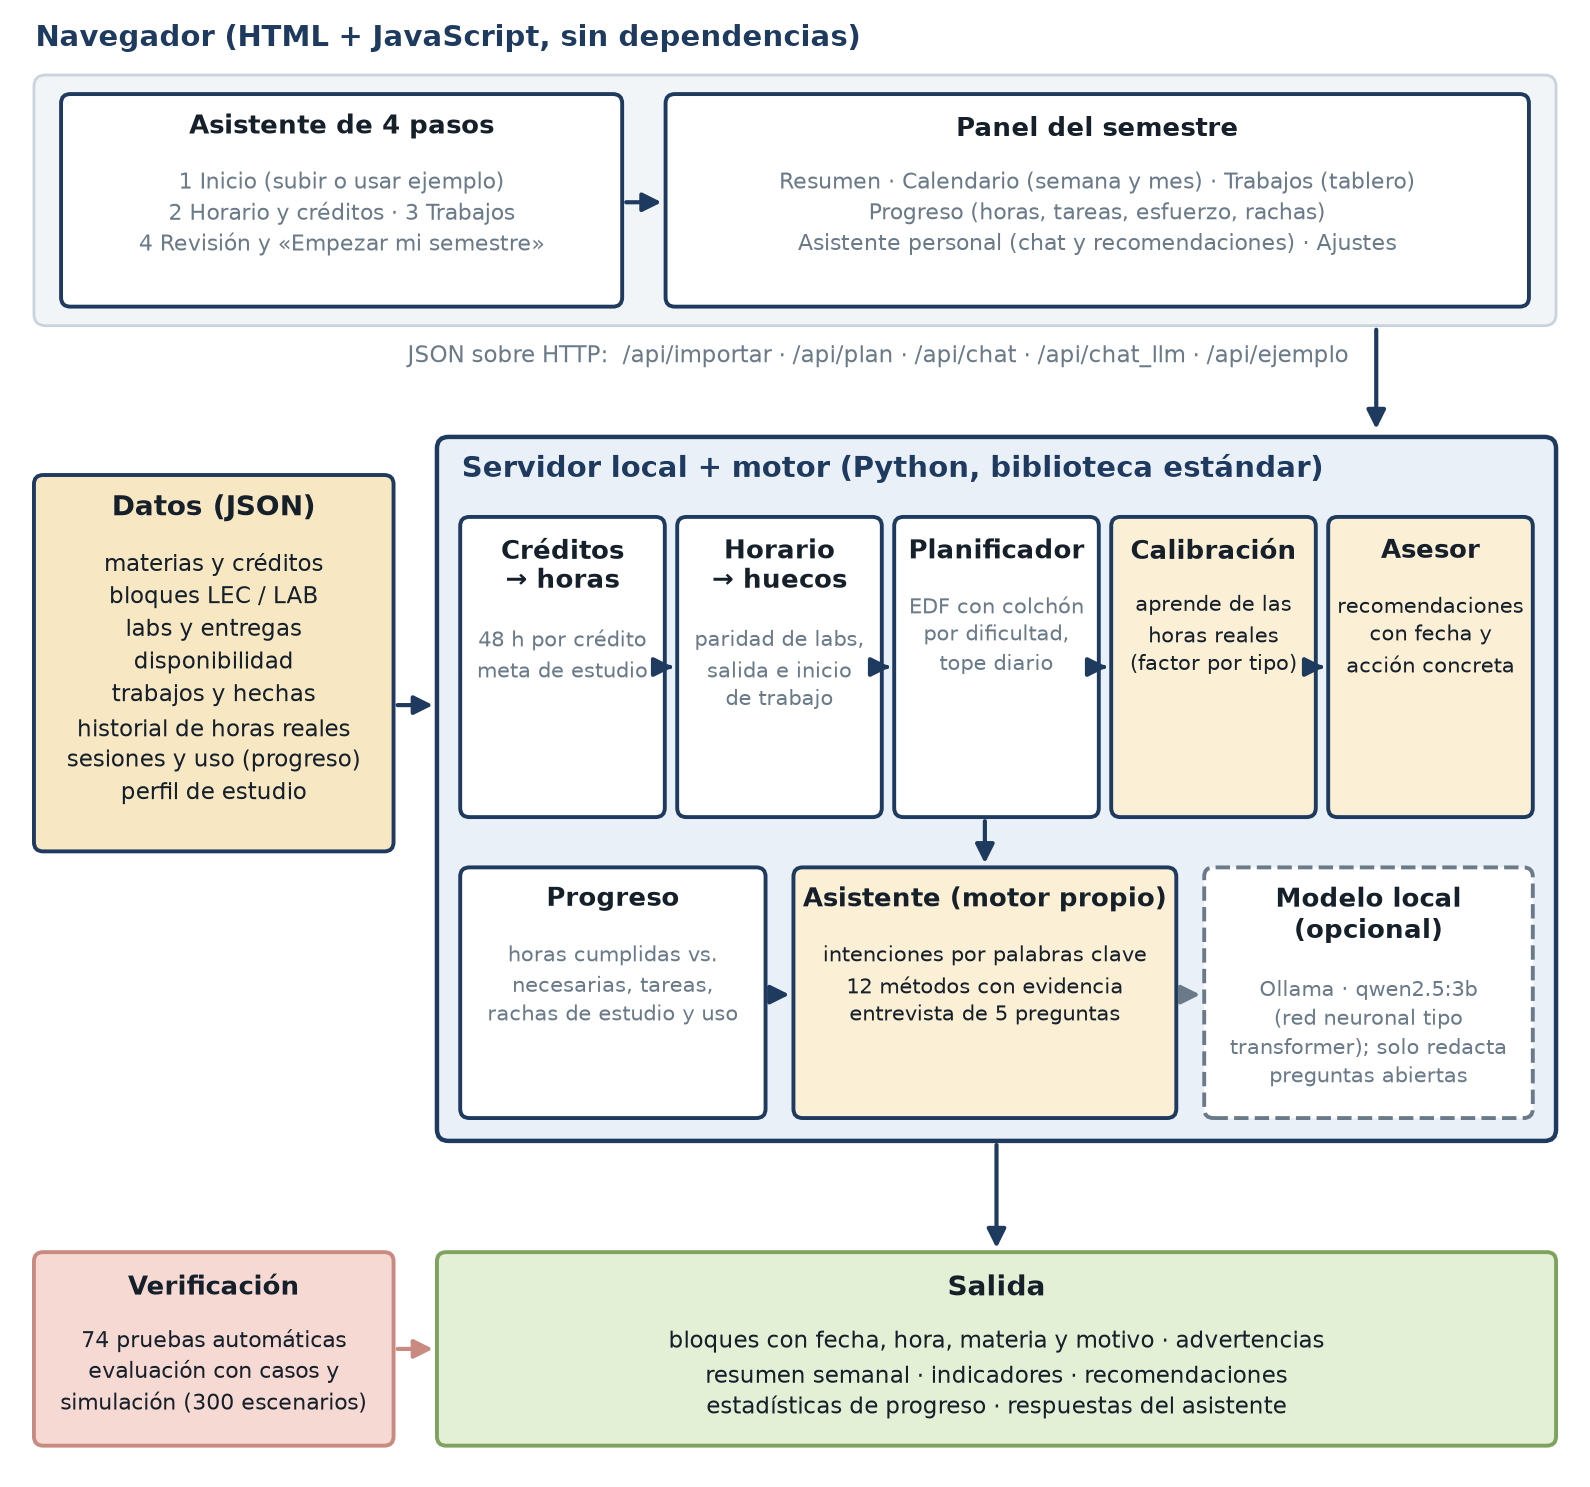
\includegraphics[width=\textwidth]{img/arquitectura.png}
\caption{Arquitectura del MVP: interfaz web, servidor local y motor de recomendación}\label{fig:arquitectura}
\end{figure}

\begin{table}[H]
\centering\small
\caption{Componentes del motor y del servidor}\label{tab:componentes}
\begin{tabularx}{\textwidth}{>{\raggedright\arraybackslash}p{4cm} >{\raggedright\arraybackslash}X}
\toprule
Componente (archivo) & Responsabilidad \\
\midrule
Motor de planificación (\texttt{motor/semestria.py}) & Créditos a horas, huecos, entregas automáticas, planificador EDF, advertencias y resumen semanal \\
Calibración (\texttt{motor/calibracion.py}) & Factor por tipo de trabajo aprendido de las horas reales \\
Asesor (\texttt{motor/asesor.py}) & Validación de horarios importados, recomendaciones e indicadores \\
Asistente (\texttt{motor/asistente.py}) & Detección de intenciones, respuestas sobre el horario, base de 12 métodos de estudio con evidencia, entrevista y plan personal, y puente opcional al modelo local \\
Progreso (\texttt{motor/progreso.py}) & Horas cumplidas, planeadas y necesarias por semana, tareas terminadas y rachas \\
Servidor (\texttt{servidor.py}) & Sirve la interfaz y expone \texttt{GET /api/ejemplo}, \texttt{POST /api/importar} (valida y normaliza un horario) y \texttt{POST /api/plan} (devuelve plan, recomendaciones, indicadores, calibración y progreso), además de \texttt{POST /api/chat}, \texttt{POST /api/chat\_llm} y \texttt{GET /api/asistente\_estado} para el asistente \\
Interfaz (\texttt{prototipo/}) & Asistente de cuatro pasos y panel con resumen, calendario, tablero de trabajos, progreso, asistente personal y ajustes \\
Datos (\texttt{datos/}) & Horario real del estudiante usado como ejemplo \\
\bottomrule
\end{tabularx}
\end{table}

\subsection{Componente principal: el planificador}

El planificador (función \texttt{planificar}) transforma los datos en el plan. La figura~\ref{fig:algoritmo} resume sus pasos y la lista siguiente (P1 a P6) los detalla.

\begin{figure}[H]
\centering
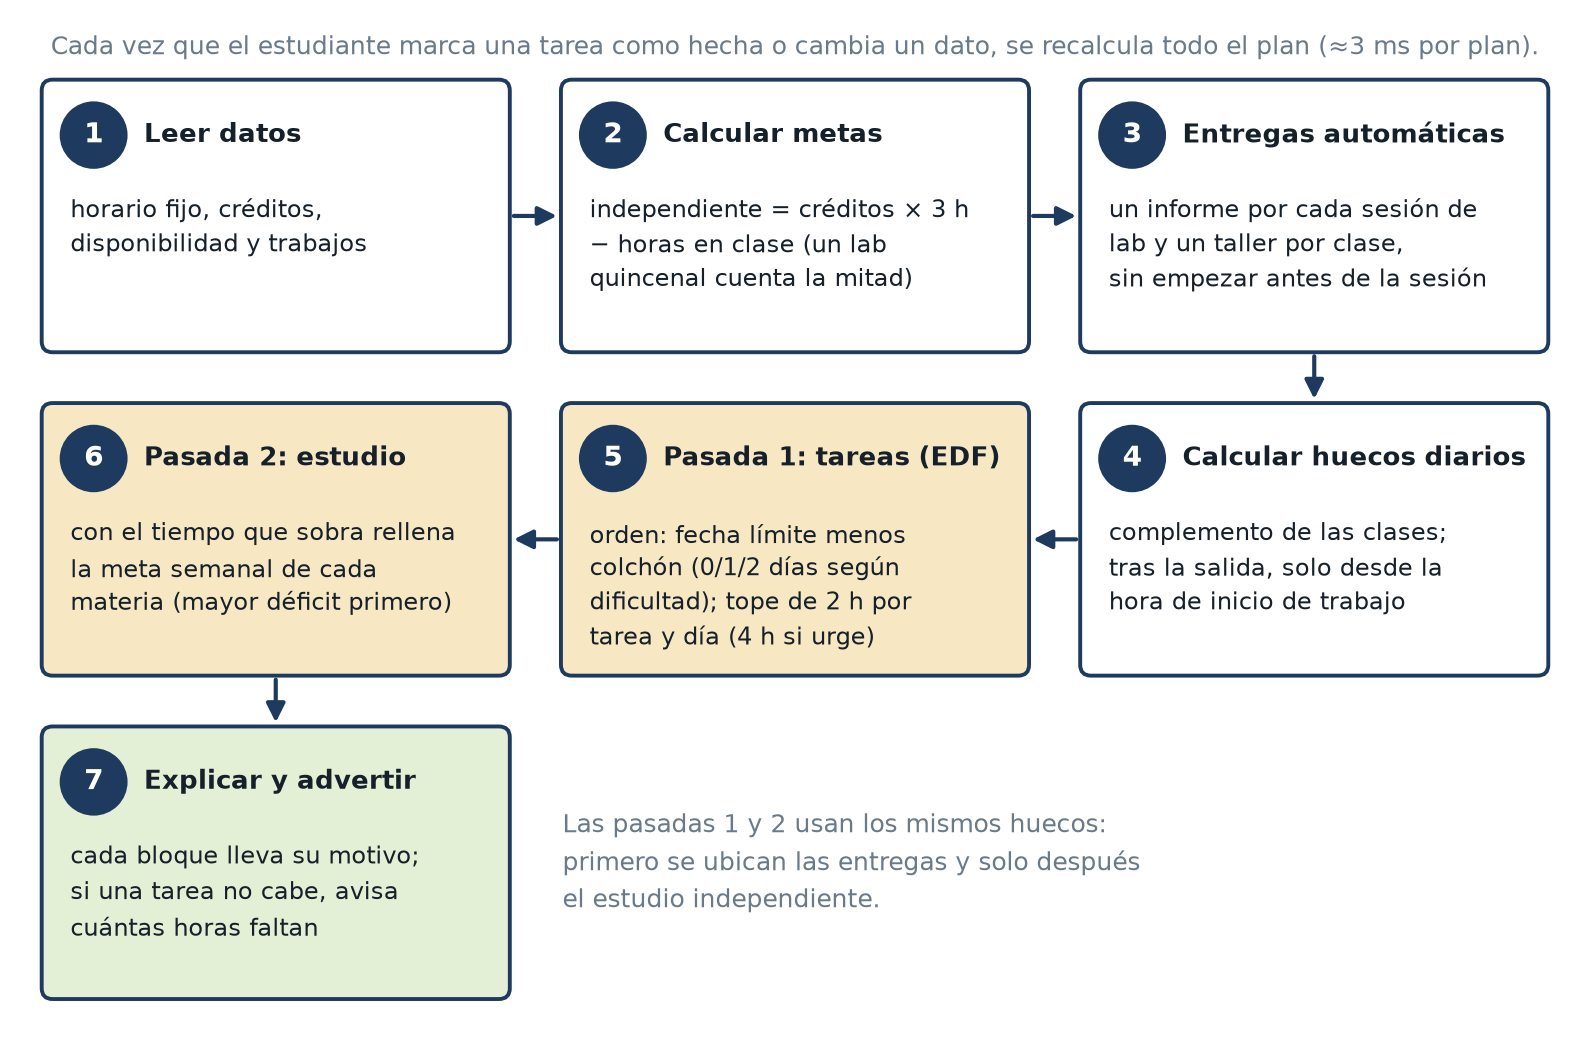
\includegraphics[width=\textwidth]{img/algoritmo.png}
\caption{Pasos del algoritmo de recomendación}\label{fig:algoritmo}
\end{figure}

\begin{enumerate}[label=\textbf{P\arabic*.}, leftmargin=*]
    \item \textbf{Leer y calcular metas.} Obtener el horizonte (hasta el domingo de la segunda semana siguiente, o la última entrega registrada) y las metas de estudio independiente por materia.
    \item \textbf{Armar las tareas.} Unir los trabajos pendientes del estudiante con los informes de laboratorio y talleres de clase que se derivan del horario (cada uno solo puede empezar después de la sesión que lo origina), con sus horas estimadas y calibradas.
    \item \textbf{Calcular los huecos de cada día.} Para cada día del horizonte, restar las clases de la franja de 7:00 a 21:00; tras la última clase solo cuenta lo que queda a partir de la hora en que el estudiante puede empezar a trabajar; descartar huecos menores a 1 hora, los días no disponibles y el tiempo ya transcurrido hoy.
    \item \textbf{Pasada 1: tareas.} Recorrer cada hueco en pasos de 30 minutos mientras no se alcance el tope diario. Entre las tareas candidatas (con tiempo pendiente, dentro de su plazo y sin superar el tope por tarea y día) elegir la de menor prioridad $p(t)$ y asignarle un bloque de 1 a 2 horas, o lo que le falte si es menos.
    \item \textbf{Pasada 2: estudio independiente.} Con el tiempo que sobra, completar semana por semana la meta de cada materia (descontando lo ya dedicado a sus tareas), empezando por la de mayor déficit.
    \item \textbf{Explicar y advertir.} Adjuntar a cada bloque su motivo; si una tarea quedó con tiempo pendiente, emitir la advertencia «no alcanza el tiempo» con las horas que faltan; si un trabajo ya venció, avisar.
\end{enumerate}

La tabla~\ref{tab:parametros} reúne los parámetros del algoritmo. El costo crece con el número de días del horizonte, de huecos por día y de tareas; en la evaluación (sección~\ref{sec:resultados}) cada plan tarda en promedio \resMsMedia\ ms.

\begin{table}[H]
\centering\small
\caption{Parámetros del planificador (valores por defecto)}\label{tab:parametros}
\begin{tabular}{ll}
\toprule
Parámetro & Valor \\
\midrule
Horas base por tipo (taller, laboratorio, proyecto, parcial) & 2 h, 3 h, 6 h, 5 h \\
Factor por dificultad (fácil, medio, difícil) & 0,75; 1; 1,5 \\
Margen antes de la entrega (fácil, medio, difícil) & 0, 1, 2 días \\
Franja de trabajo & 7:00 a 21:00 \\
Tope de trabajo por día & 6 h \\
Tope por tarea y día & 2 h (4 h si la entrega es en $\leq$ 1 día) \\
Bloque mínimo y máximo & 60 y 120 min (paso de 30 min) \\
Hueco mínimo aprovechable & 60 min \\
\bottomrule
\end{tabular}
\end{table}

\begin{table}[H]
\centering\footnotesize
\caption{Ejemplo del plan generado para el lunes 12 y el martes 13 de octubre (caso base); cada bloque lleva su motivo}\label{tab:ejemplo}
\begin{tabularx}{\textwidth}{l l >{\raggedright\arraybackslash}p{4.6cm} >{\raggedright\arraybackslash}X}
\toprule
Día & Hora & Bloque & Motivo \\
\midrule
lunes 12/10 & 09:00--11:00 & Taller MATE ECDI (06/10) & Se entrega mañana (13/10). Por su dificultad (medio) se planea con 1 día de margen. Al ser inminente, se permiten hasta 4 h hoy en esta tarea. \\
lunes 12/10 & 11:00--12:30 & Taller CIENCBAS ASTO (06/10) & Se entrega mañana (13/10). Dificultad fácil. Al ser inminente, se permiten hasta 4 h hoy en esta tarea. \\
lunes 12/10 & 12:30--14:30 & Informe de laboratorio ISIS ARSW (09/10) & Se entrega en 4 días (16/10). Por su dificultad (difícil) se planea con 2 días de margen. Se reparte en bloques de máximo 2 h por día. \\
martes 13/10 & 07:00--09:00 & Informe de laboratorio ISIS ARSW (09/10) & Se entrega en 3 días (16/10). Por su dificultad (difícil) se planea con 2 días de margen. Se reparte en bloques de máximo 2 h por día. \\
martes 13/10 & 09:00--11:00 & Informe de laboratorio ISIS PTIA (10/10) & Se entrega en 4 días (17/10). Dificultad fácil. Se reparte en bloques de máximo 2 h por día. \\
martes 13/10 & 17:00--19:00 & Parcial 2 de ECDI & Se entrega en 7 días (20/10). Por su dificultad (difícil) se planea con 2 días de margen. Se reparte en bloques de máximo 2 h por día. \\
\bottomrule
\end{tabularx}
\end{table}


\subsection{Asistente personal y módulo de progreso}\label{sec:asistente}

Además del plan, el MVP incluye un \textbf{asistente personal} en forma de chat y una sección de \textbf{progreso}. La sección de recomendaciones dejó de ser una lista de textos: ahora son tarjetas por categoría (foco, riesgo, estrategia, carga, bienestar, estudio y progreso) y, al tocar una, el chat la explica con pasos, fechas del plan del estudiante, gráficas sencillas y la evidencia que la respalda; luego la persona puede preguntar.

\textbf{Flujo de una consulta.} (1) El mensaje se normaliza (minúsculas, sin tildes). (2) Se detecta la intención por coincidencia de raíces de palabras, con puntaje; si una pregunta mezcla un método de estudio con una intención de horario, gana el método salvo que se pregunte por hoy, mañana o ahora. (3) Un manejador consulta el plan, las tareas y las estadísticas y arma la respuesta como una lista de \emph{bloques} tipados (párrafo, lista, línea de tiempo, barras con línea de límite, ciclo de enfoque y pausa, plantilla copiable y evidencia) que la interfaz dibuja. (4) Se ofrecen preguntas sugeridas. Si ninguna intención aplica y hay un modelo local disponible, la pregunta pasa a la capa opcional descrita en la sección~\ref{sec:tipo-ia}.

\textbf{Qué responde.} Preguntas sobre el horario (qué hay hoy o mañana, qué sigue, próximas entregas, si va atrasado, cuándo está libre, créditos y horas de estudio, calibración y progreso), cómo prepararse para un parcial y métodos de estudio y bienestar. También hace una \textbf{entrevista de cinco preguntas} (mejor momento del día, cómo estudia, qué lo distrae, cuántas horas duerme y su mayor reto) con la que arma un \textbf{plan de estudio personal}: unas reglas eligen los métodos que corresponden al perfil y los ubican en los huecos de su plan (figura~\ref{fig:perfil}).

\textbf{Base de métodos.} El asistente solo recomienda métodos incluidos en una base propia de doce temas, cada uno con qué es, por qué funciona, pasos y referencias (tabla~\ref{tab:metodos}). Cuando una convención no tiene sustento científico, el texto lo dice (por ejemplo, que los 25 minutos de la técnica Pomodoro son una costumbre útil y no una regla científica).

\begin{table}[H]
\centering\small
\caption{Métodos de estudio y bienestar de la base del asistente}\label{tab:metodos}
\begin{tabularx}{\textwidth}{>{\raggedright\arraybackslash}p{4.6cm} >{\raggedright\arraybackslash}X >{\raggedright\arraybackslash}p{3.6cm}}
\toprule
Método & Idea central & Evidencia \\
\midrule
Práctica de recuperación & Recordar sin mirar en lugar de releer & \cite{Roediger2006,Dunlosky2013} \\
Repetición espaciada & Repartir los repasos en varios días & \cite{Cepeda2006,Dunlosky2013} \\
Práctica intercalada & Mezclar tipos de problema en una sesión & \cite{Rohrer2007,Dunlosky2013} \\
Autoexplicación & Explicar el tema con palabras propias & \cite{Chi1994,Dunlosky2013} \\
Bloques de enfoque con pausas & Pausas breves para sostener la atención & \cite{Ariga2011} \\
Planes «si\dots entonces\dots» & Definir de antemano cuándo y dónde empezar & \cite{Gollwitzer2006} \\
Cómo arrancar cuando se posterga & Reducir el costo de empezar & \cite{Steel2007} \\
Dormir como parte del estudio & Proteger el sueño antes de una prueba & \cite{Curcio2006} \\
Movimiento y pausas activas & Actividad física regular & \cite{Hillman2008} \\
Celular fuera de la vista & Reducir distracciones durante el bloque & \cite{Ward2017} \\
Manejar los nervios & Escribir las preocupaciones antes de la prueba & \cite{Ramirez2011} \\
Qué evitar: releer y subrayar & Técnicas de baja utilidad & \cite{Dunlosky2013} \\
\bottomrule
\end{tabularx}
\end{table}

Estos estudios describen efectos promedio en poblaciones concretas; el asistente los presenta como orientación y no como garantía de un resultado individual, y ante nervios intensos recomienda buscar apoyo profesional.

\textbf{Progreso.} La sección de progreso se alimenta de lo que el estudiante registra: bloques marcados como cumplidos, las horas reales que anota al terminar un trabajo y los días en que abre la aplicación. Para cada semana calcula tres cantidades: las horas \emph{necesarias}, que salen de los créditos ($\sum_{m}\max(0,\,3c_m-h_{clase,m})$ sobre las materias $m$); las horas \emph{planeadas}, que son las que el plan le propone; y las horas \emph{cumplidas}, que son las registradas. Con ellas se muestran el porcentaje de la meta, un gráfico de las últimas ocho semanas, el avance por materia, las tareas terminadas por semana, un mapa de actividad de 35 días y dos rachas: de estudio (días seguidos con horas registradas) y de uso. La racha actual no se rompe si hoy todavía no hay actividad, para no castigar al estudiante a mitad del día. Las figuras~\ref{fig:progreso} y~\ref{fig:asistente} muestran ambas pantallas con datos de ejemplo.

\begin{figure}[H]
\centering
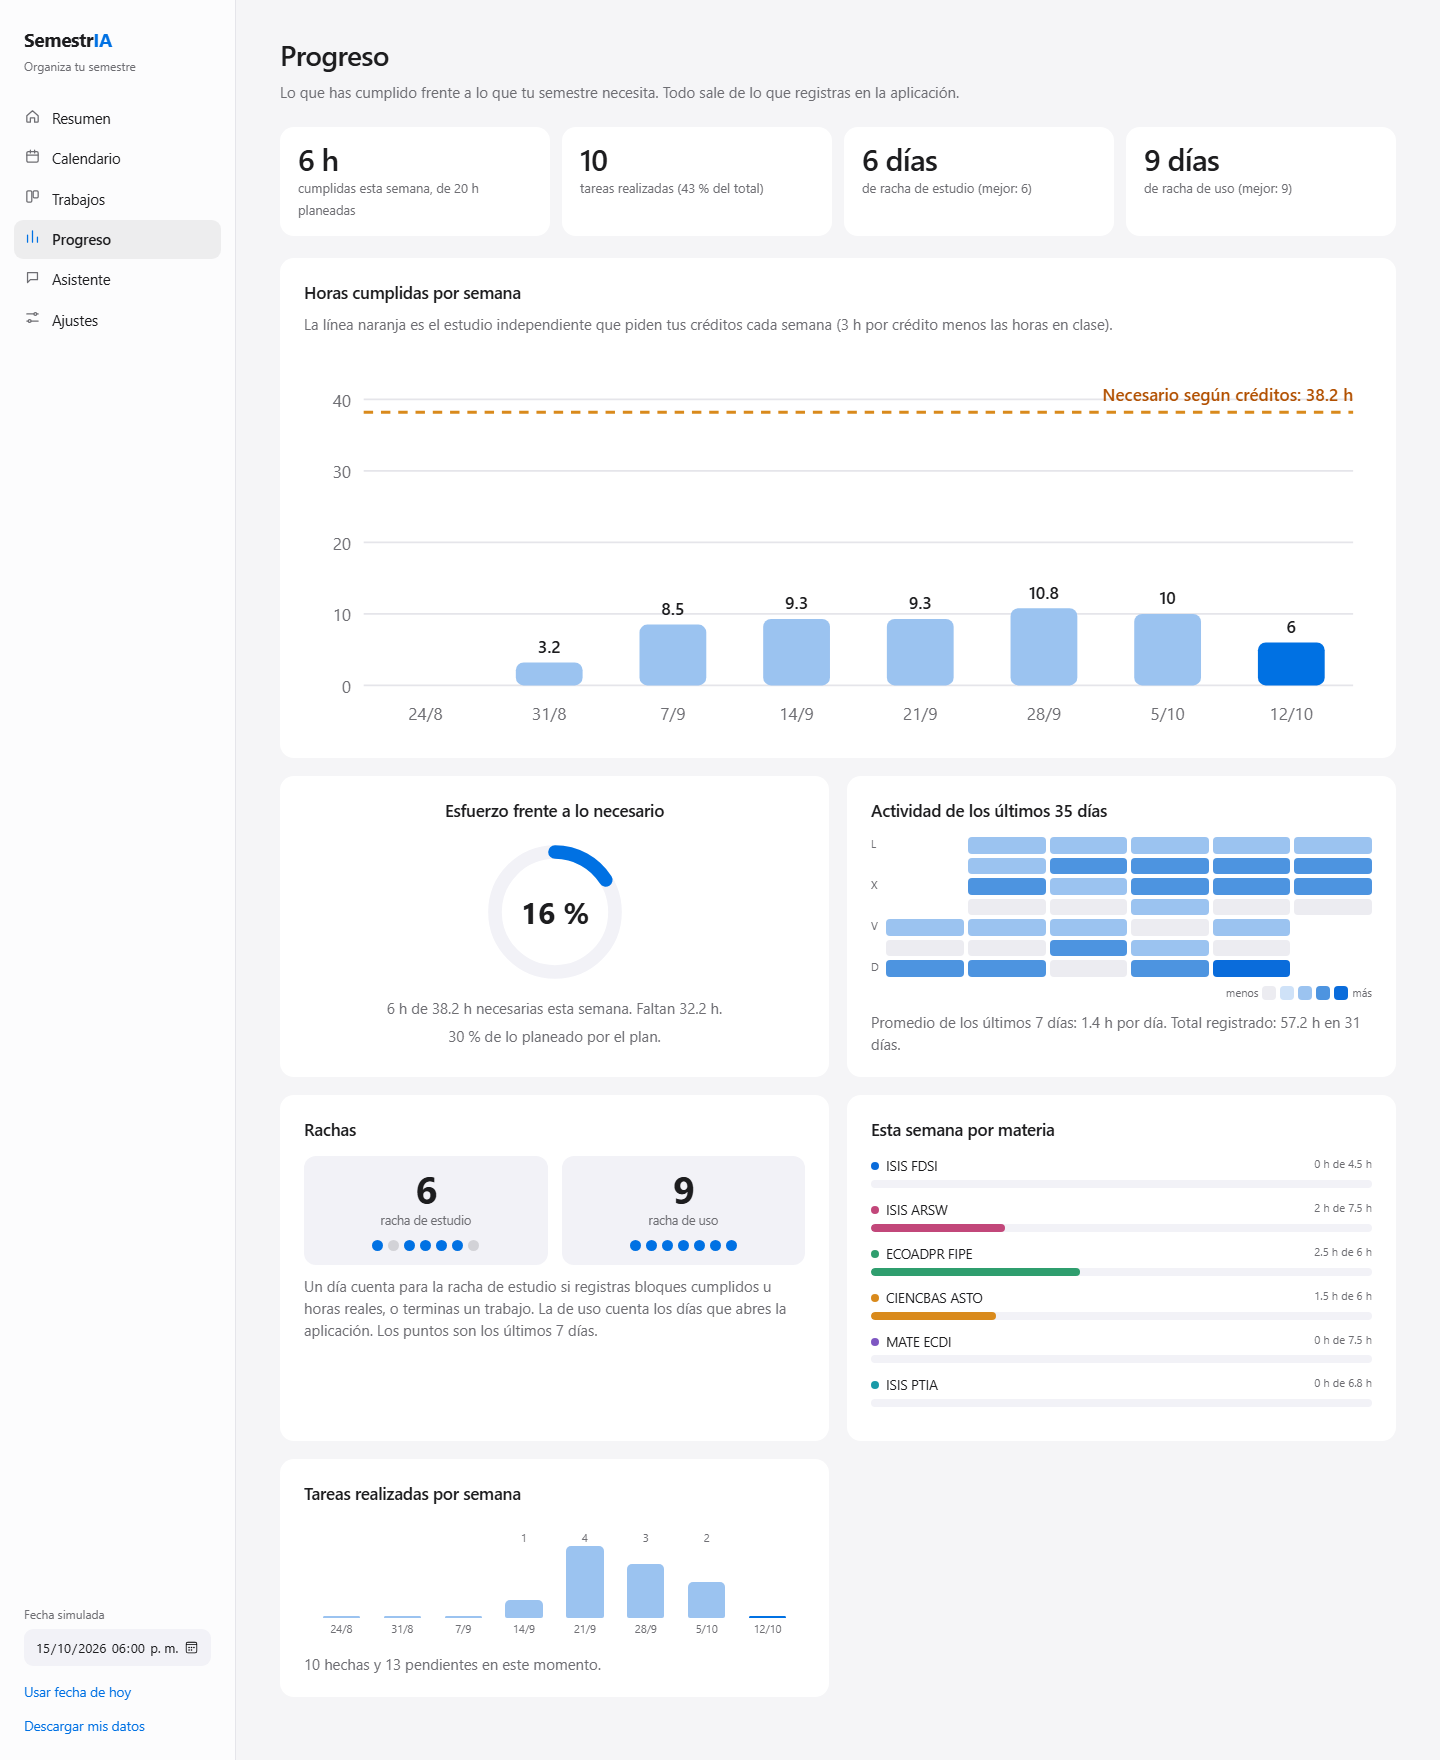
\includegraphics[width=\textwidth]{img/pant_09_progreso.png}
\caption{Progreso: horas cumplidas frente a las necesarias, tareas realizadas, mapa de actividad y rachas (datos de demostración)}\label{fig:progreso}
\end{figure}

\begin{figure}[H]
\centering
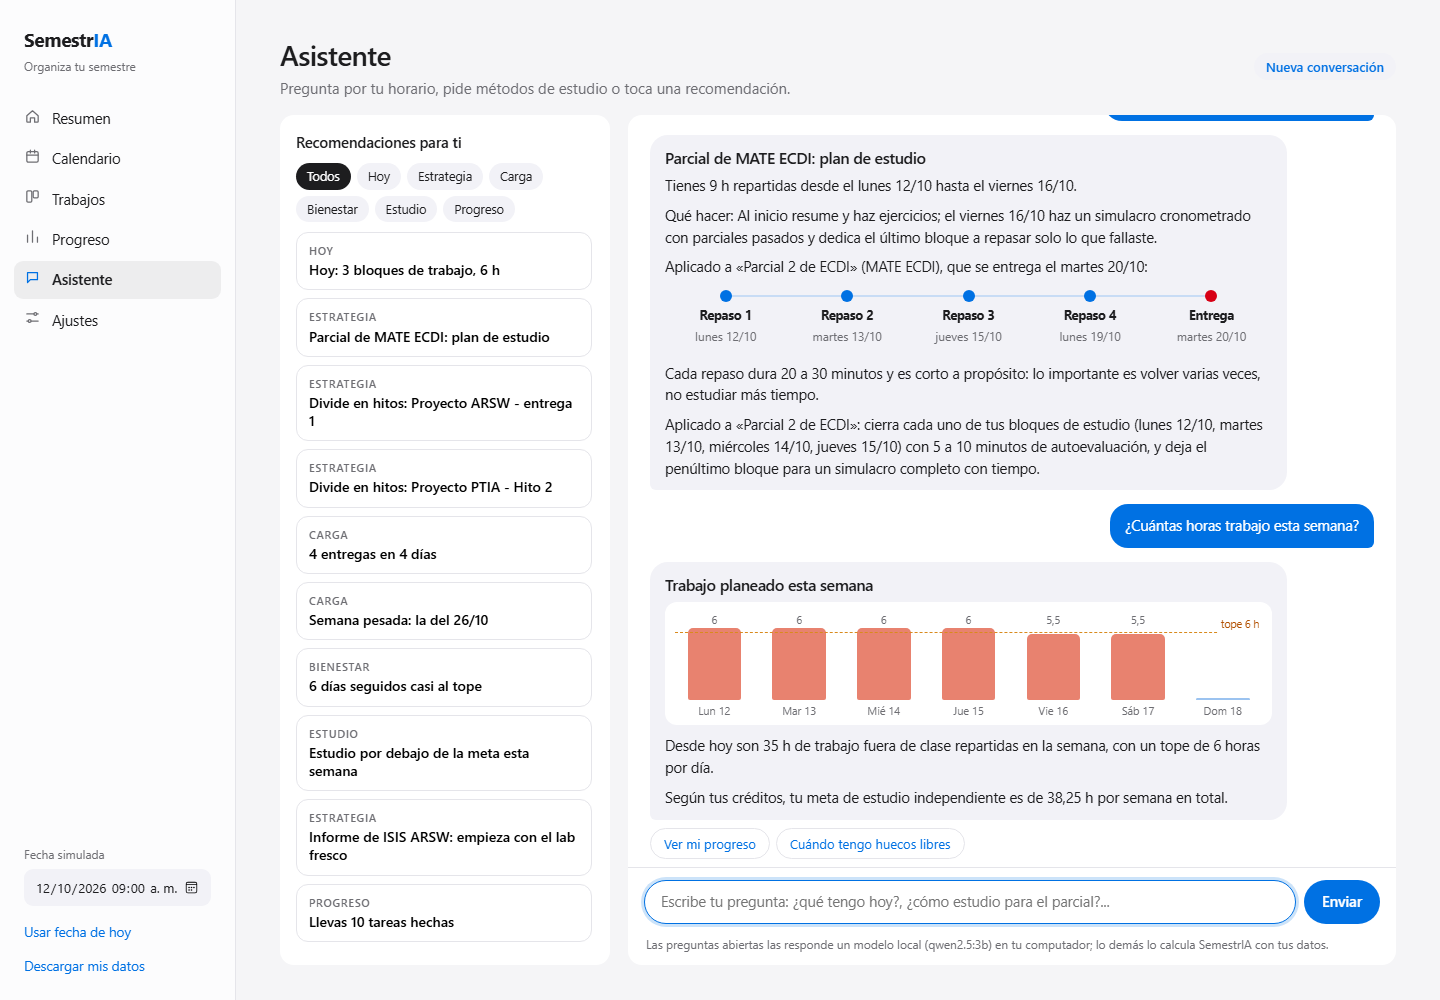
\includegraphics[width=\textwidth]{img/pant_10_asistente.png}
\caption{Asistente personal: recomendaciones por categoría y chat que las explica (datos de demostración)}\label{fig:asistente}
\end{figure}

\begin{figure}[H]
\centering
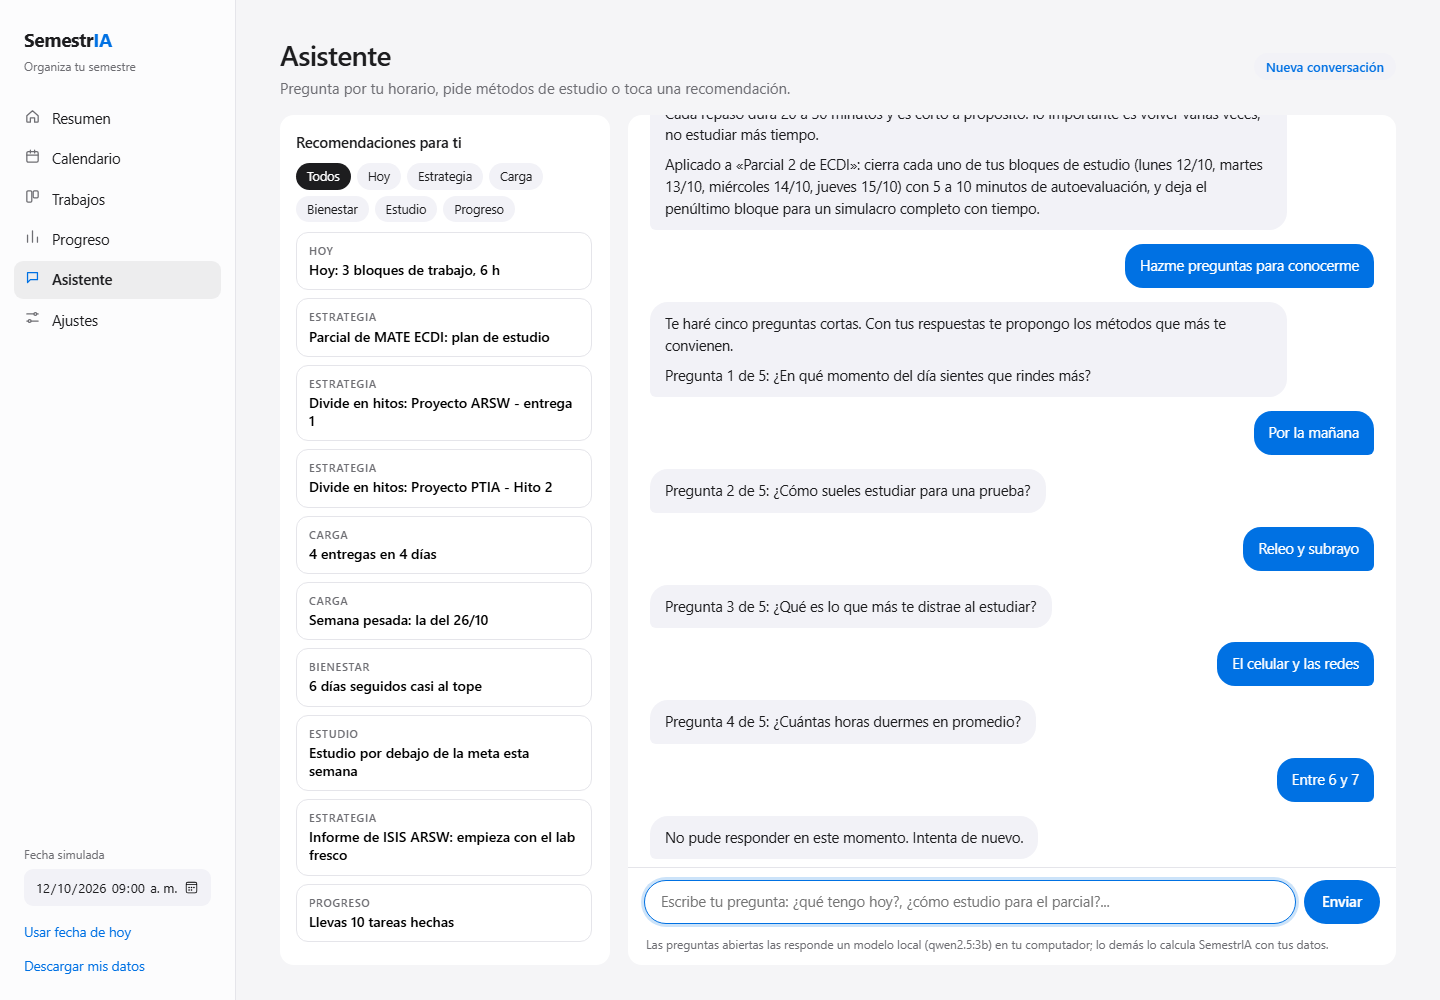
\includegraphics[width=\textwidth]{img/pant_11_asistente_perfil.png}
\caption{Entrevista de cinco preguntas y plan de estudio personal}\label{fig:perfil}
\end{figure}


\subsection{Interfaz del MVP}

La interfaz evolucionó desde el prototipo en papel del Hito 1 y el prototipo navegable del Hito 2 hasta un MVP con funciones reales. Se organiza en dos momentos. Primero, un \textbf{asistente de cuatro pasos} (inicio, horario y créditos, trabajos y revisión final) que termina con el botón «Empezar mi semestre», que fija el horario. Después, un \textbf{panel} con las secciones resumen, calendario, trabajos, progreso, asistente personal y ajustes (las dos últimas se describen en la sección~\ref{sec:asistente}). Las figuras~\ref{fig:revision} a~\ref{fig:tablero} muestran las pantallas principales con los datos de ejemplo (con un trabajo en curso y uno hecho).

\begin{figure}[H]
\centering
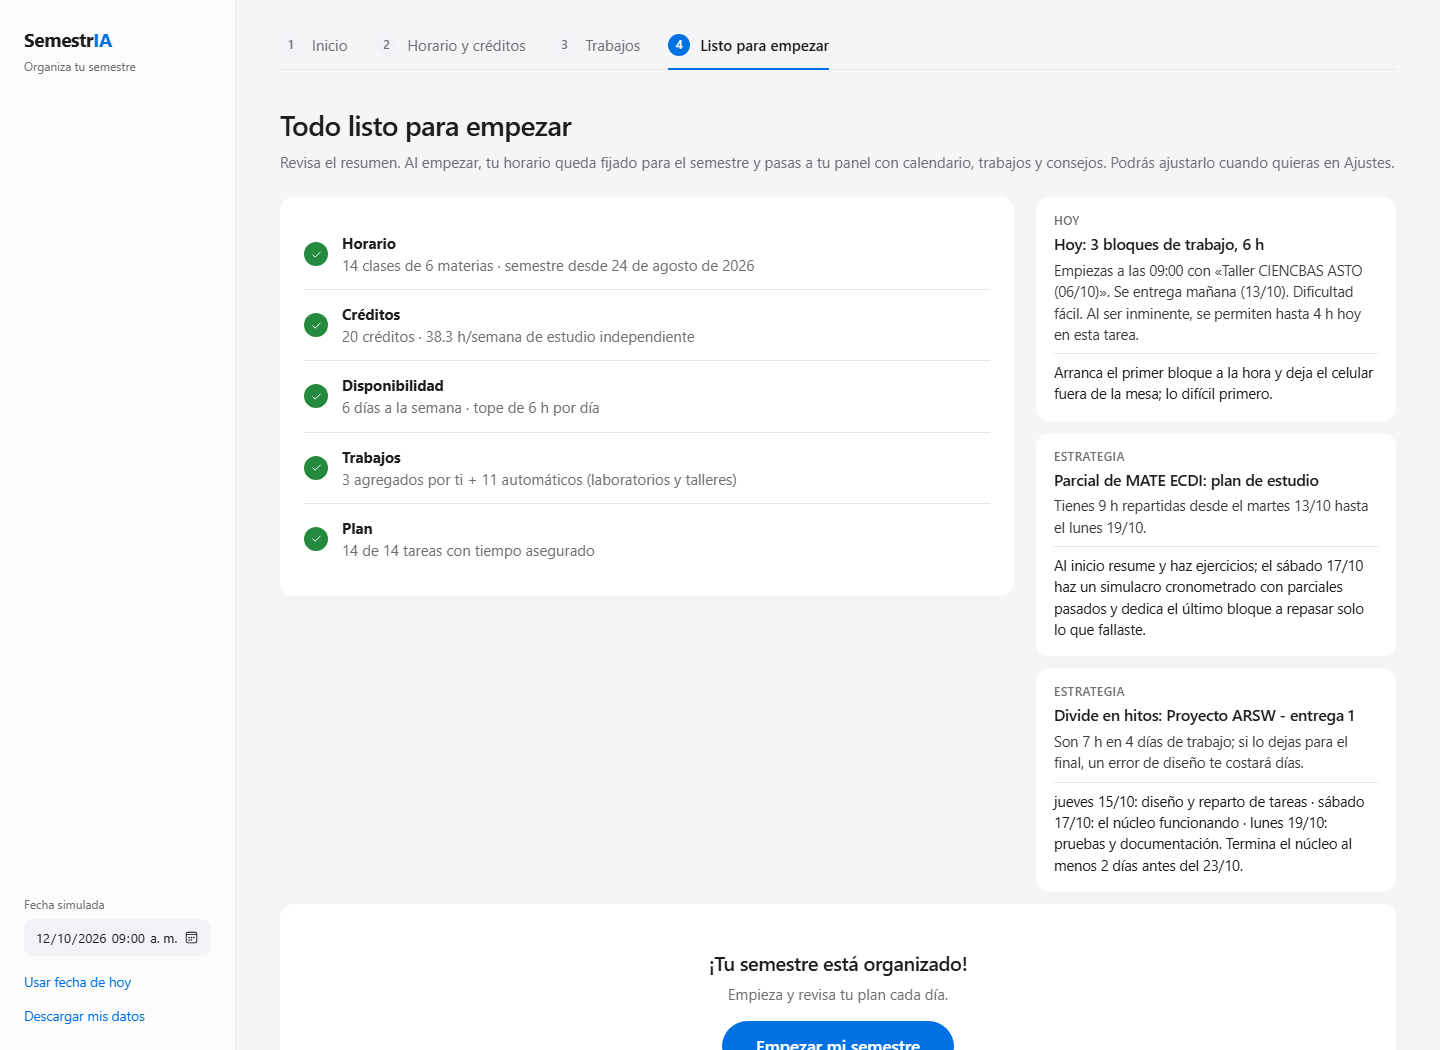
\includegraphics[width=\textwidth]{img/pant_04_revision_final.png}
\caption{Último paso del asistente: revisión y botón «Empezar mi semestre»}\label{fig:revision}
\end{figure}

\begin{figure}[H]
\centering
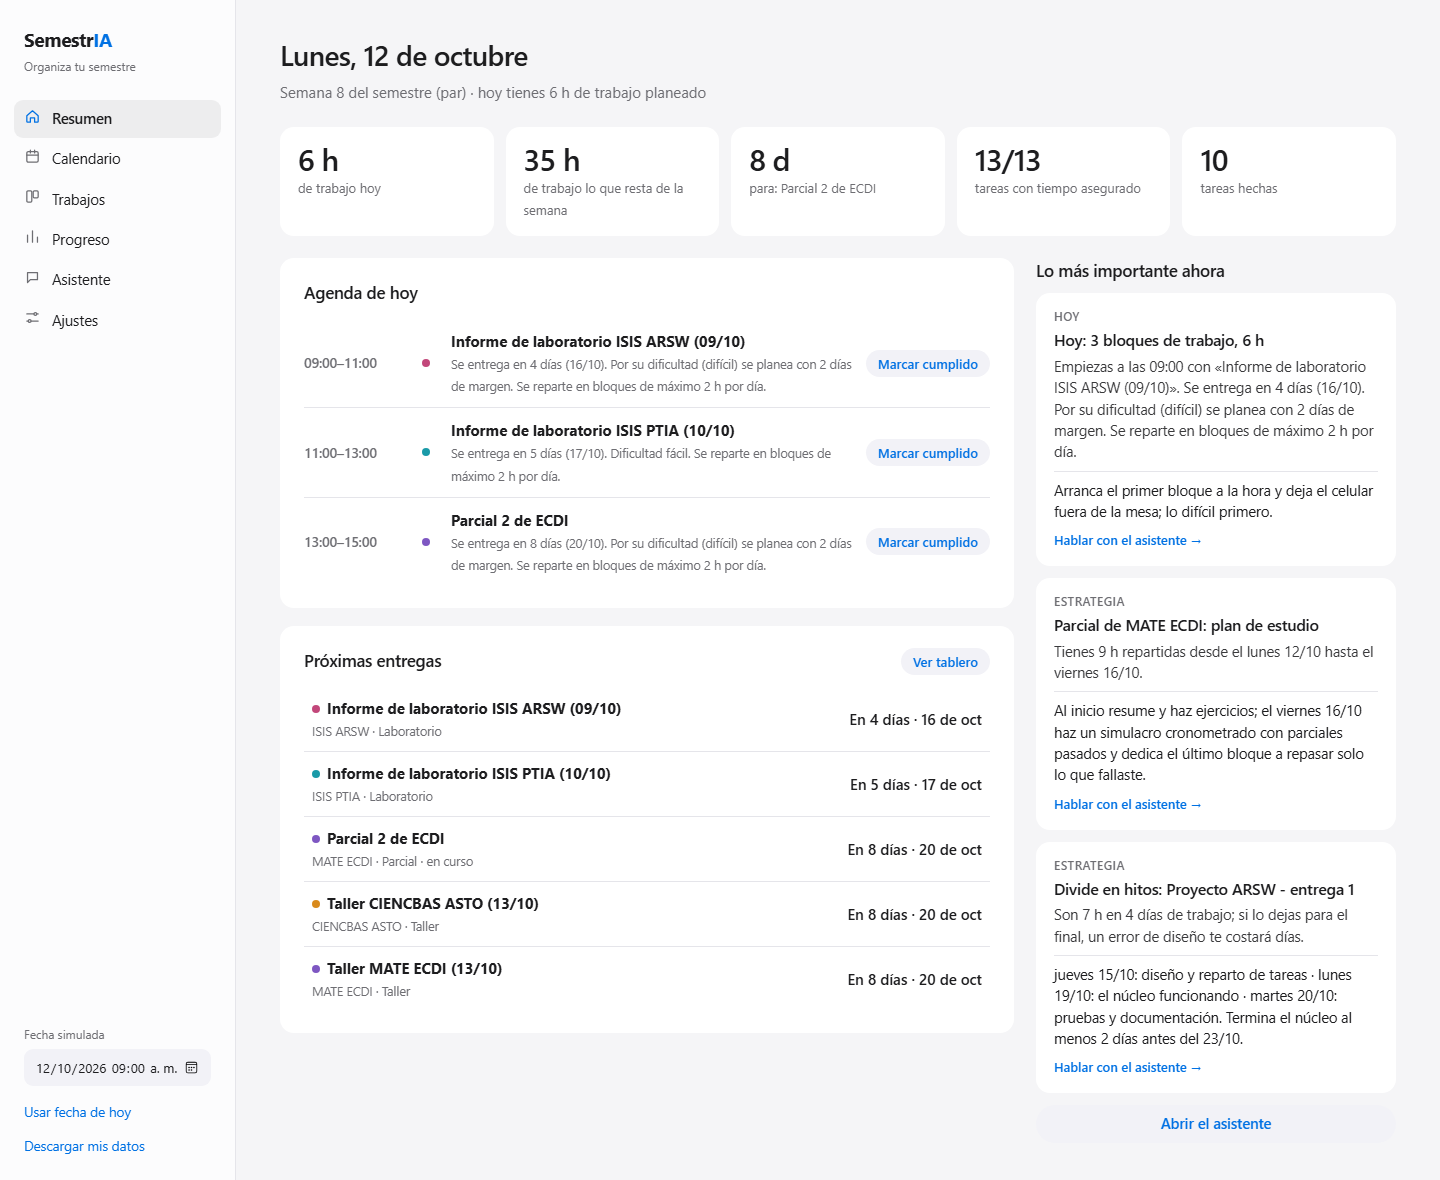
\includegraphics[width=\textwidth]{img/pant_05_resumen.png}
\caption{Resumen: agenda de hoy, indicadores, próximas entregas y recomendaciones}\label{fig:resumen}
\end{figure}

\begin{figure}[H]
\centering
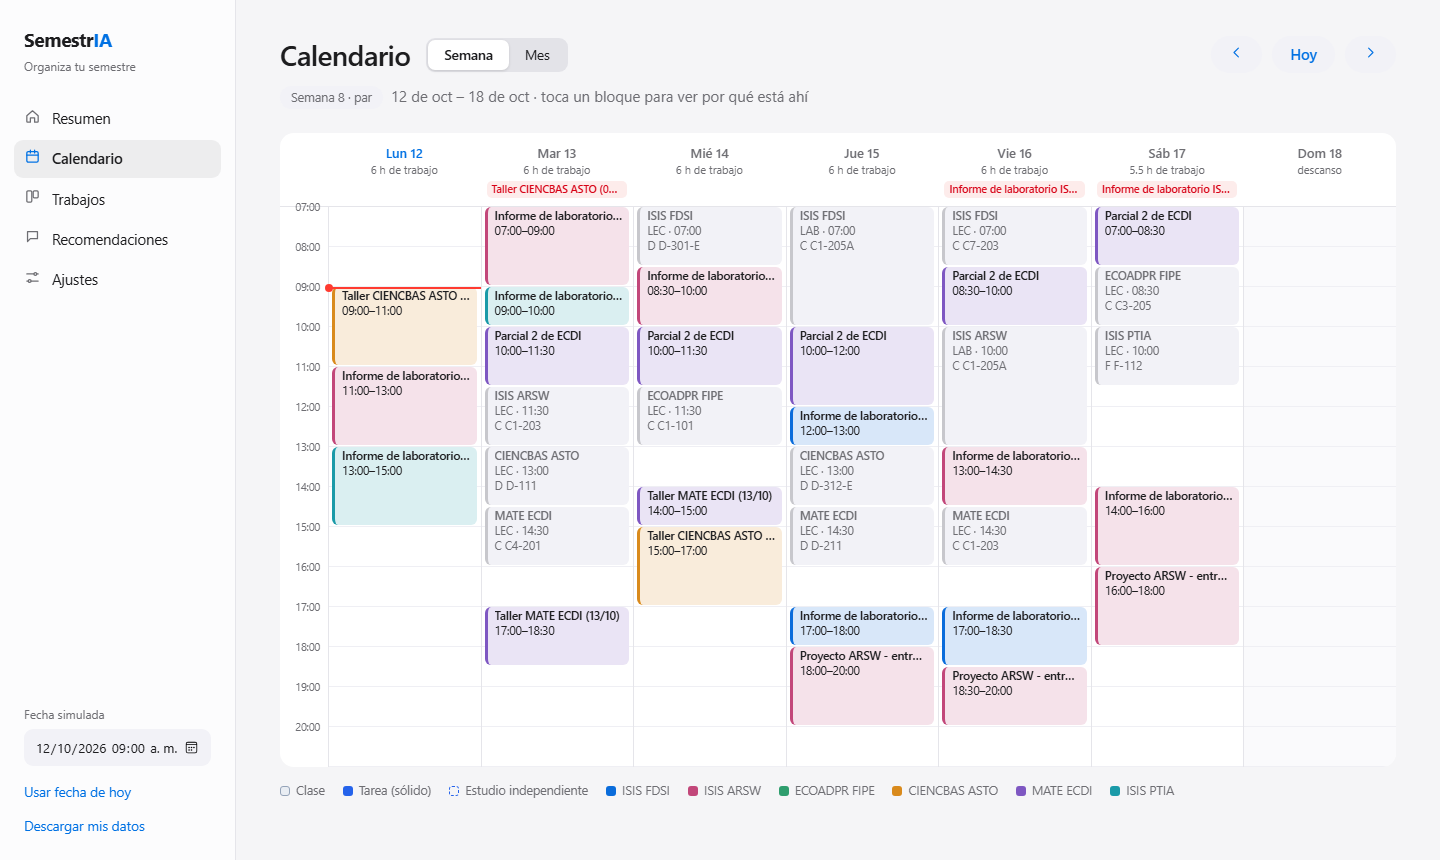
\includegraphics[width=\textwidth]{img/pant_06_calendario_semana.png}
\caption{Calendario semanal con clases, tareas, estudio y entregas}\label{fig:calendario}
\end{figure}

\begin{figure}[H]
\centering
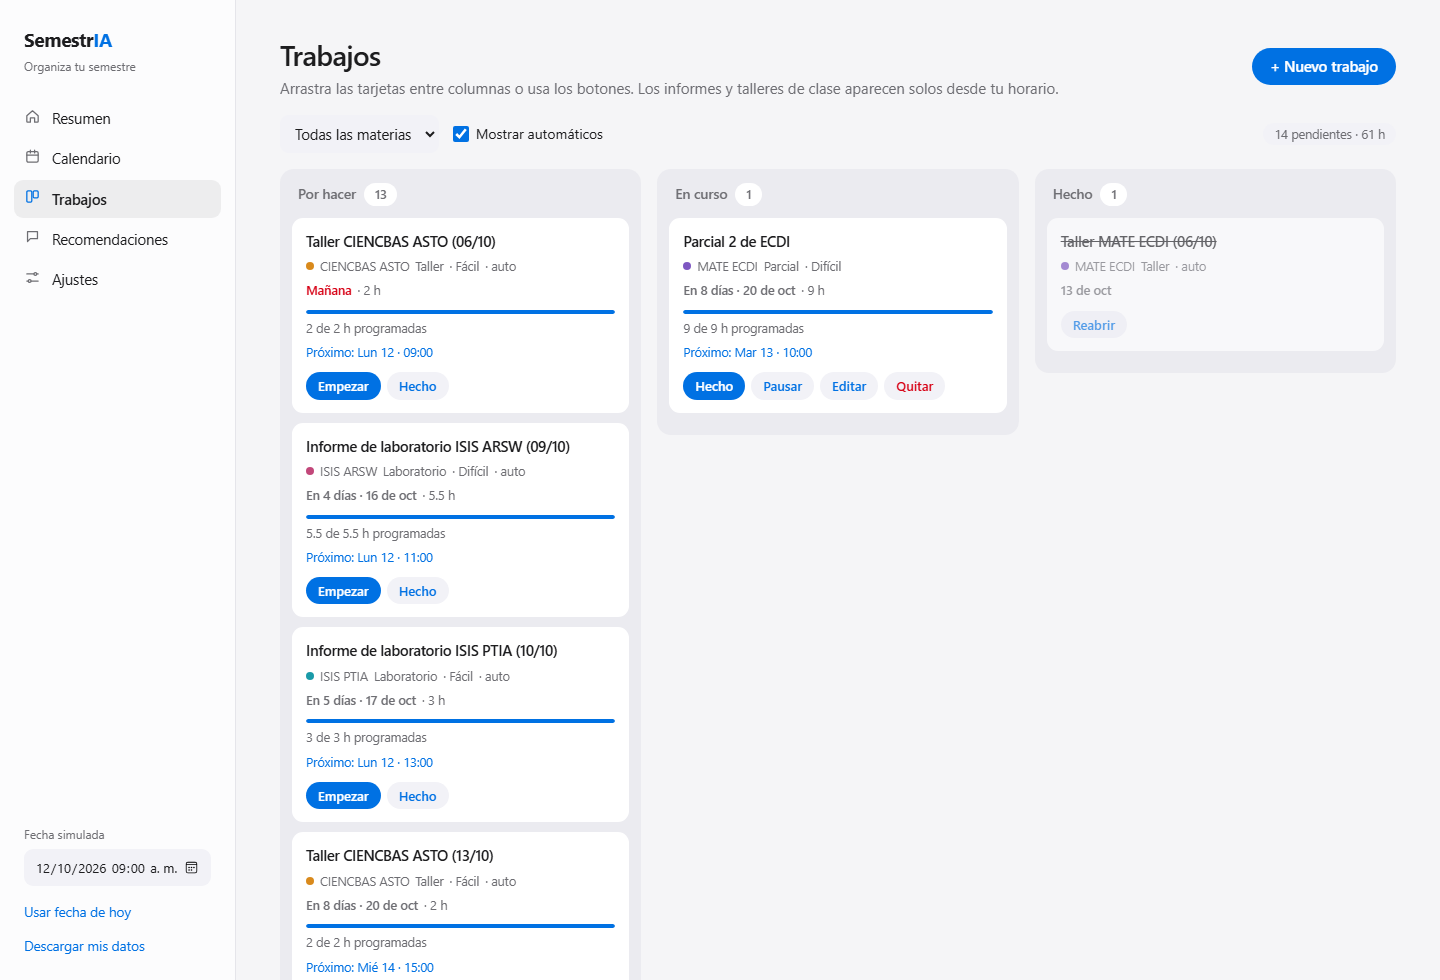
\includegraphics[width=\textwidth]{img/pant_08_trabajos_tablero.png}
\caption{Tablero de trabajos: por hacer, en curso y hecho}\label{fig:tablero}
\end{figure}

\subsection{Consideraciones éticas}

\begin{itemize}
    \item \textbf{Autonomía.} El sistema recomienda, y la persona decide: puede editar horas, fechas y disponibilidad, marcar trabajos como hechos o ignorar el plan.
    \item \textbf{Privacidad.} Todo se ejecuta en el computador del estudiante; el horario y los trabajos no se envían a terceros, ni siquiera al modelo de lenguaje opcional, que también corre en local, y el estado se guarda en el propio navegador. El estudiante puede descargar o borrar sus datos.
    \item \textbf{Salud y consejos.} El asistente da orientación general de estudio y bienestar, no consejos médicos ni psicológicos; ante nervios intensos remite a bienestar universitario o a un profesional. Los métodos citan estudios, pero sus efectos son promedios y no garantías.
    \item \textbf{Bienestar.} Los topes diarios, los márgenes por dificultad y los días sin disponibilidad evitan jornadas excesivas; el asesor advierte cuando hay días seguidos casi al tope.
    \item \textbf{Transparencia.} Cada bloque dice por qué está donde está, cada recomendación explica qué detectó y qué hacer, y la calibración muestra el factor aprendido.
    \item \textbf{Honestidad sobre los límites.} Cuando algo no cabe, el sistema lo dice y propone alternativas en lugar de ocultarlo.
\end{itemize}

\subsection{Fuentes del diseño y del código}

\begin{itemize}
    \item \textbf{Código:} escrito por el estudiante; usa solo la biblioteca estándar de Python y JavaScript del navegador, sin bibliotecas de terceros. Se reparte en el motor (\texttt{motor/}), el servidor (\texttt{servidor.py}), la interfaz (\texttt{prototipo/}) y las pruebas (\texttt{pruebas/}); el anexo~\ref{anexo:estructura} muestra la estructura y cómo ejecutarlo.
    \item \textbf{Datos:} \texttt{datos/horario\_ejemplo.json} es el horario real del estudiante; los créditos de algunas materias son supuestos.
    \item \textbf{Fuentes del diseño:} la equivalencia entre créditos y horas viene de la norma colombiana \parencite{MEN2019}; el orden por fecha límite, de la teoría de planificación \parencite{Liu1973,Russell2021}; la distinción entre restricciones duras y blandas, de la literatura de horarios \parencite{Schaerf1999}. Las horas base por tipo de trabajo y los márgenes por dificultad son \textbf{supuestos propios}, sin calibrar con datos externos; para eso existe el módulo de calibración.
    \item \textbf{Fuentes del asistente:} los métodos de estudio y bienestar proceden de la literatura citada en la tabla~\ref{tab:metodos}; las reglas que los eligen según el perfil son propias. La capa opcional usa un modelo de terceros preentrenado (Qwen2.5 mediante Ollama) sin modificarlo.
    \item \textbf{Historial:} el prototipo navegable del Hito 2 (con una réplica del motor en JavaScript) se conserva en la carpeta \texttt{archivo\_hito2/}.
\end{itemize}
